\subsection{Algorithms and Techniques}
%Algorithms and techniques used in the project are thoroughly discussed and properly justified based on the characteristics of the problem.

In this task, I'll use Convolutional Neural Network(CNN). CNN has been successful in  practical applications for image recognition.CNN consists of convolution layer, pooling layer and fully-connected layer and sometimes contains local contrast normalization(LCN). In this chapter, I'll discuss the convolution layer and pooling.
As the name 'convolution' suggests, the network employs a mathematical operation called convolution. \cite{Deep Learning}\cite{Deep Learning2}

Fig.5 is the example of the architecture of the CNN.Fig.6 illustrates the image of the CNN.\cite{Machine Learning}

\begin{figure}[htbp]

	\begin{center}
	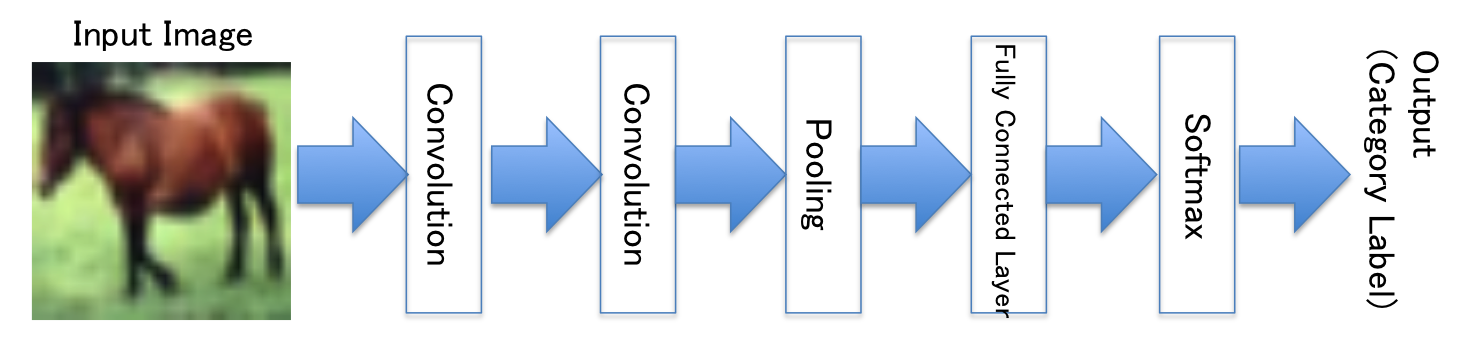
\includegraphics[width=10cm]{picture/Architecture_of_CNN.png}
	\caption{An example of CNN Architecture}
	\end{center}
	\label{fig:five}

\end{figure}



\begin{figure}[htbp]

	\begin{center}
	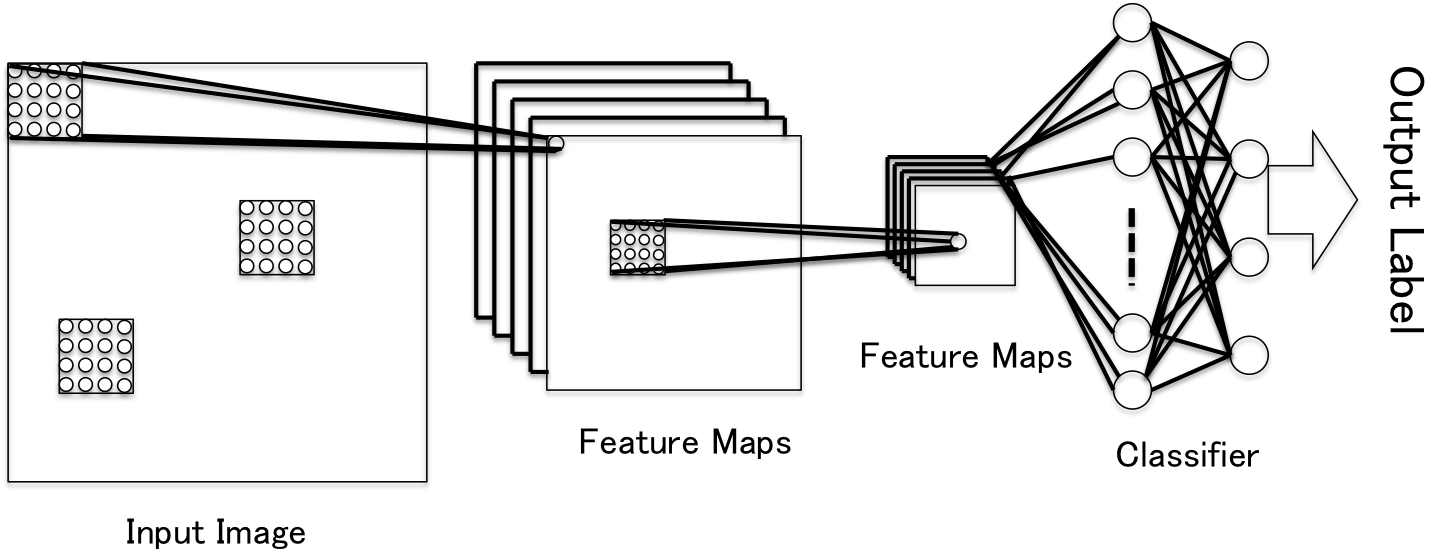
\includegraphics[width=10cm]{picture/Structure_of_convolution.png}
	\caption{Overview of CNN}
	\end{center}
	\label{fig:six}

\end{figure}

\begin{figure}[H]

	\begin{center}
	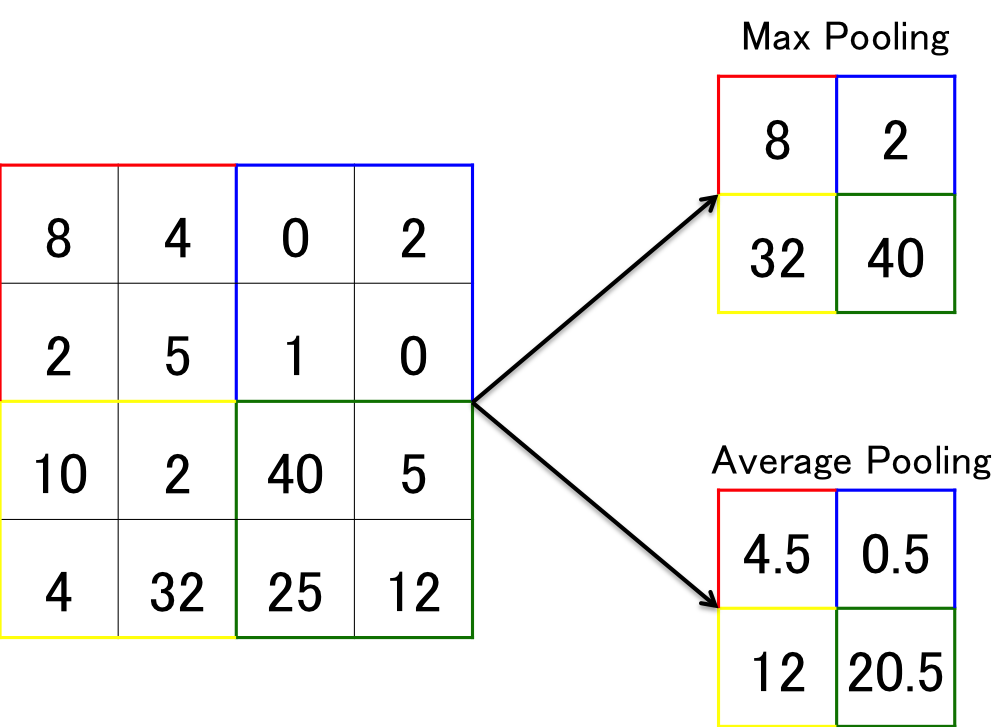
\includegraphics[width=10cm]{picture/Pooling.png}
	\caption{Example of Max Pooling and Average Pooling}
	\end{center}
	\label{fig:seven}

\end{figure}

 



%\begin{itemize}
% \item 3D volumes of neurons\\
 %The layers of a CNN have neurons arranged in 3 dimensions: width,height and weight. The neurons inside a layer are only connected to a small region of the layer before it which is so called 'receptive field'.
 %\item Local Connectivity\\
 %This is the most distinguishing feature of CNN. Typical multilayer perceptron are densely connected. Because of the connectivity,  we can't utilize the architecture for image recognition because of the curse of dimensionality. As for CNN, the connectivity are inspired by the neuro-science(visual cortex). Therefore, the dimensionality is much smaller than the typical multilayer perceptron. The CNN architecture ensures that the learnt "filters" produce the strongest response to a spatially local input pattern. Stacking many such layers leads to non-linear "filters" that become increasingly "global". Because of this, the network can create good representations of small parts of input, then assemble representations of large areas from them.
 %\item Shared weights\\
 %Each filter is replicated across the entire visual field in CNN. These replicated units share the same parameterization and form a feature map. Since the parameters are shared, the number of free parameters decrease. Therefore, when running CNNs model, the memory use will decrease, which means we can train more powerful(more layers) networks.
%\end{itemize}

Convolutional neural networks are biologically inspired variants of multilayer perceptron.They are emulated by the behavior of a visual cortex.\cite{cnn}\
In the convolutional layer, the input images are convolved by filters. This process is basically the same as the convolution of the general image processing which convolves small size image into the input image so that the image gets blur or emphasizes edge.

To be more specific, the input image has S$\times$S for each channel and 2D filter has L$\times$L.
The input image are convolved by the 2D filter for each channel and then each result are added. Suppose input image can be written as $x_{ijk} ((i,j,k)\in [0,S-1]\times[0,S-1]\times[1,N])$ and the calculation result is $u_{ij}$ and as for the filter, I define $w_{ijk} ((i,j,k)\in[0,L-1]\times[0,L-1]\times[1,N])$.
The output will be as follows.

\begin{eqnarray}
u_{ij}=\sum_{k=1}^{N}\biggl[\sum_{(p,q)\in P_{ij}}x_{pqk}w_{p-i,q-j,k}\biggl]+b_{k}
\end{eqnarray}

$P_{ij}$ is the $L\times L$ square area whose center is $(i,j)$ and $b_{k}$is the bias.

\begin{eqnarray}
P_{ij}=\{(i+i^{'},j+j^{'})| i^{'}=0,...,L-1,j^{'}=0,...,L-1\}
\end{eqnarray}

When the input image size is large, the stride of filter will be larger than 1.However, in this case, some features won't be captured. Therefore, the performance will decline in general.\
After this convolutional process, $u_{ij}$ pass through the activation function, then the output will be produced.
\begin{eqnarray}
y_{ij}=a(u_{ij})
\end{eqnarray}
If the number of the filter is $N^{'}$, the output dimension will be $y_{ijk} ((i,j,k)\in[0,S-1]\times [0,S-1]\times [1,N^{'}])$

Pooling layer is put after the convolution layer. %Pooling layer reduces the dimensionality of the input image. 
The function of the pooling layer is to progressively reduce the spatial size of the representation to reduce the amount of parameters and computation in the network, and hence to also control overfitting.
By introducing pooling layer, not only the architecture will be more robust but also the dimensionality will be reduced. Max pooling and Average pooling are the typical pooling which are generally utilized. Figure.7 is the example of the pooling.The original map is the size of 4$\times$4. The stride for the pooling is 2 and the pooling size is 2$\times$2. "Max pooling" is to extract the maximum pixel from each region and "Average pooling" is to calculate the average value for each region.In this task, I utilized max pooling at the pooling layers.


